\section{Referencia del Archivo /media/docs/progra/c++/compiladores1/proy2/godzilla/src/ast.c}
\label{ast_8c}\index{/media/docs/progra/c++/compiladores1/proy2/godzilla/src/ast.c@{/media/docs/progra/c++/compiladores1/proy2/godzilla/src/ast.c}}
Implementacion del arbol de sintaxis abstracta. 

{\tt \#include $<$stdio.h$>$}\par
{\tt \#include $<$stdlib.h$>$}\par
{\tt \#include $<$string.h$>$}\par
{\tt \#include \char`\"{}ast.h\char`\"{}}\par


Dependencia gr\'{a}fica adjunta para ast.c:\begin{figure}[H]
\begin{center}
\leavevmode
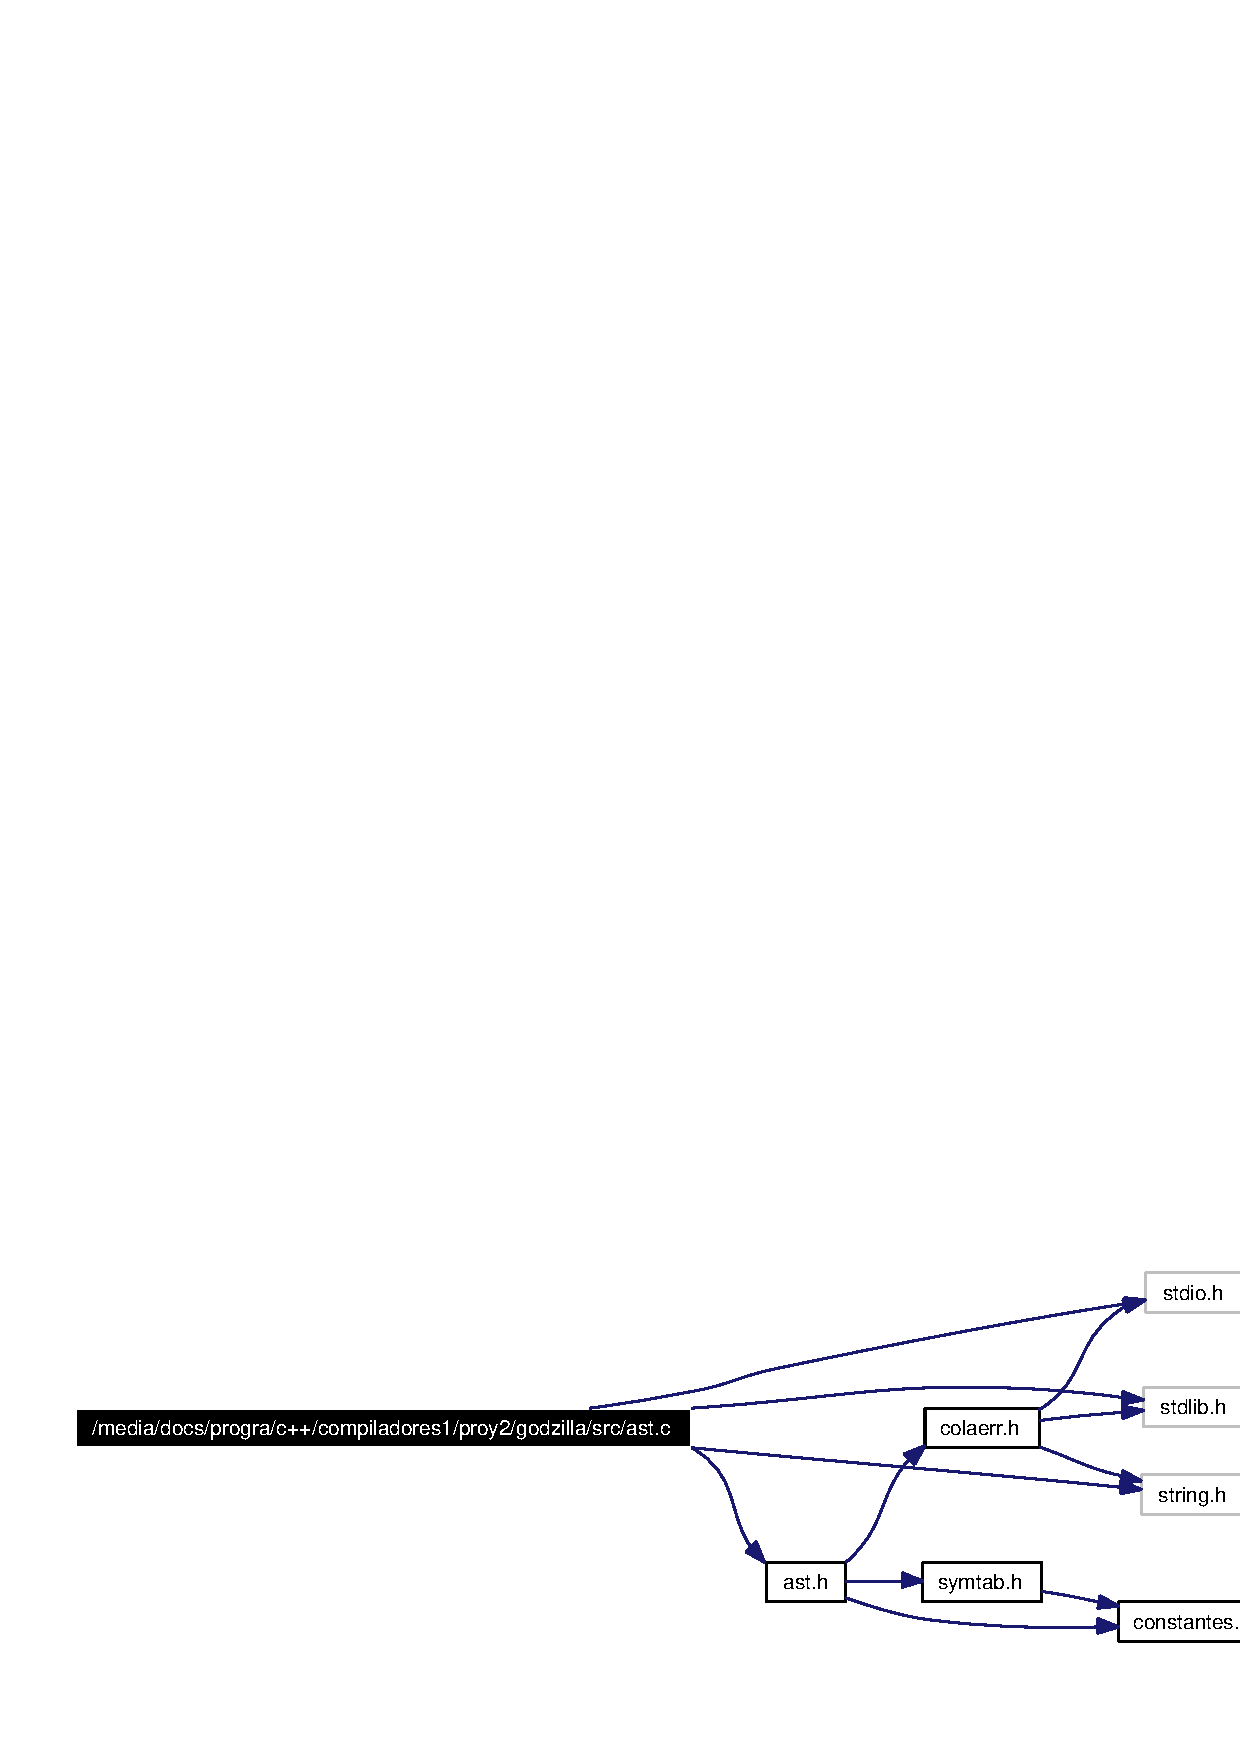
\includegraphics[width=305pt]{ast_8c__incl}
\end{center}
\end{figure}
\subsection*{Funciones}
\begin{CompactItemize}
\item 
{\bf nodo} $\ast$ {\bf ref\-Nodo\-Hijo} (int tipo, void $\ast$dato)
\begin{CompactList}\small\item\em Crea un nodo que refiere al nodo recien creado para sea utilizado por el nodo anterior a este. \item\end{CompactList}\item 
{\bf nodo} $\ast$ {\bf insertar\-Constante} (int tipo, int dato)
\begin{CompactList}\small\item\em Agrega una constante al arbol de expresiones. \item\end{CompactList}\item 
{\bf nodo} $\ast$ {\bf insertar\-Variable} (char $\ast$ident)
\begin{CompactList}\small\item\em Agrega una variable al arbol de expresiones. \item\end{CompactList}\item 
{\bf nodo} $\ast$ {\bf insertar\-Cadena} (char $\ast$cadena)
\begin{CompactList}\small\item\em Agrega una cadena al arbol de expresiones. \item\end{CompactList}\item 
{\bf nodo} $\ast$ {\bf insertar\-Operacion} (int operador, {\bf nodo} $\ast$l, {\bf nodo} $\ast$r)
\begin{CompactList}\small\item\em Inserta una operacion al arbol de expresiones. \item\end{CompactList}\item 
{\bf nodo} $\ast$ {\bf insertar\-Expresion} ({\bf nodo} $\ast$n)
\begin{CompactList}\small\item\em Agrega un nuevo arbol de expresiones al arbol principal. \item\end{CompactList}\item 
{\bf nodo} $\ast$ {\bf insertar\-Asignacion} (char $\ast$identificador, {\bf nodo} $\ast$expresion)
\begin{CompactList}\small\item\em Agrega una asignacion al arbol principal. \item\end{CompactList}\item 
{\bf nodo} $\ast$ {\bf insertar\-Sentencia} (int tipo, {\bf nodo} $\ast$n, int nlinea)
\begin{CompactList}\small\item\em agrega una sentencia al arbol principal \item\end{CompactList}\item 
{\bf nodo} $\ast$ {\bf concatenar\-Sentencia} ({\bf nodo} $\ast$n1, {\bf nodo} $\ast$n2)
\begin{CompactList}\small\item\em Concatena sentencias para caminar por estas. \item\end{CompactList}\item 
{\bf nodo} $\ast$ {\bf insertar\-Declaracion} (char $\ast$identificador, int tipo\-Dato)
\begin{CompactList}\small\item\em agrega una nuva declaracion al arbol principal \item\end{CompactList}\item 
{\bf nodo} $\ast$ {\bf insertar\-Enunciado\-If} ({\bf nodo} $\ast$expresion, {\bf nodo} $\ast$nthen, {\bf nodo} $\ast$nelse)
\begin{CompactList}\small\item\em Agrega un nuevo enunciado if al arbol de sentencias. \item\end{CompactList}\item 
{\bf nodo} $\ast$ {\bf insertar\-Ciclo\-While} ({\bf nodo} $\ast$expresion, {\bf nodo} $\ast$stmt)
\begin{CompactList}\small\item\em Agrega un nuevo ciclo while ar arbol de sentecias. \item\end{CompactList}\item 
{\bf nodo} $\ast$ {\bf insertar\-Ciclo\-For} (char $\ast$idx, int asig, int lim, {\bf nodo} $\ast$body)
\begin{CompactList}\small\item\em Agrega un nuevo ciclo for al arbol de sentencias. \item\end{CompactList}\item 
{\bf nodo} $\ast$ {\bf insertar\-Token} (int tipo, void $\ast$dato)
\begin{CompactList}\small\item\em Agrega un nuevo token al arbol de sentencias. \item\end{CompactList}\item 
{\bf nodo} $\ast$ {\bf concatenar\-Tokens} ({\bf nodo} $\ast$t1, {\bf nodo} $\ast$t2)
\begin{CompactList}\small\item\em Concatena tokens para parametros de llamadas. \item\end{CompactList}\item 
{\bf nodo} $\ast$ {\bf insertar\-Llamada} ({\bf nodo} $\ast$n)
\begin{CompactList}\small\item\em Agrega un nueva llamada de impresion a yyout al arbol de sentencias. \item\end{CompactList}\item 
{\bf nodo} $\ast$ {\bf insertar\-Llamada\-Sym\-Tab} (int ln)
\begin{CompactList}\small\item\em Agrega un nueva llamada de impresion de tabla de simbolos al arbol de sentencias. \item\end{CompactList}\item 
void {\bf crear\-Raiz} ({\bf nodo} $\ast$n, {\bf ast} $\ast$tree)
\begin{CompactList}\small\item\em Genera el nodo raiz para el arbol dado en el segundo parametro como punto de inicio del arbol y punto de meta del recorrido sintactico. \item\end{CompactList}\item 
void {\bf error} (char $\ast$msg, int tipo, void $\ast$dato)
\begin{CompactList}\small\item\em Escribe error semantico hacia cola de errores semanticos. \item\end{CompactList}\item 
int {\bf recorrer\-Arbol} ({\bf ast} $\ast$tree, char $\ast$filename)
\begin{CompactList}\small\item\em Recorre el arbol y escribe resultado en archivo salida. \item\end{CompactList}\item 
int {\bf recorrer\-Sentencia} ({\bf sentencia} $\ast$s)
\begin{CompactList}\small\item\em Recorre sentencias recursivamente y devuelve resultado acarreado. \item\end{CompactList}\item 
int {\bf evaluar\-Sentencia} ({\bf sentencia} $\ast$s)
\begin{CompactList}\small\item\em Evalua sentencia y selecciona tipo de sentencia a evaluar. \item\end{CompactList}\item 
int {\bf evaluar\-Declaracion} ({\bf declaracion} $\ast$d)
\begin{CompactList}\small\item\em Evalua declaracion. \item\end{CompactList}\item 
int {\bf evaluar\-Asignacion} ({\bf asignacion} $\ast$a)
\begin{CompactList}\small\item\em Evalua asignacion. \item\end{CompactList}\item 
{\bf nodo} $\ast$ {\bf evaluar\-Expresion} ({\bf expr} $\ast$e)
\begin{CompactList}\small\item\em Evalua expresion y selecciona tipo de expresion a evaluar. \item\end{CompactList}\item 
{\bf nodo} $\ast$ {\bf evaluar\-Operacion} ({\bf operacion} $\ast$o)
\begin{CompactList}\small\item\em Selecciona operacion binaria a evaluar. \item\end{CompactList}\item 
{\bf nodo} $\ast$ {\bf evaluar\-And} ({\bf nodo} $\ast$n1, {\bf nodo} $\ast$n2)
\begin{CompactList}\small\item\em Evalua operacion logica AND. \item\end{CompactList}\item 
{\bf nodo} $\ast$ {\bf evaluar\-Or} ({\bf nodo} $\ast$n1, {\bf nodo} $\ast$n2)
\begin{CompactList}\small\item\em Evalua operacion logica OR. \item\end{CompactList}\item 
{\bf nodo} $\ast$ {\bf evaluar\-EQ} ({\bf nodo} $\ast$n1, {\bf nodo} $\ast$n2)
\begin{CompactList}\small\item\em Evalua operacion comparativa Igual. \item\end{CompactList}\item 
{\bf nodo} $\ast$ {\bf evaluar\-NEQ} ({\bf nodo} $\ast$n1, {\bf nodo} $\ast$n2)
\begin{CompactList}\small\item\em Evalua operacion comparativa Desigual. \item\end{CompactList}\item 
{\bf nodo} $\ast$ {\bf evaluar\-GT} ({\bf nodo} $\ast$n1, {\bf nodo} $\ast$n2)
\begin{CompactList}\small\item\em Evalua operacion comparativa Mayor Que. \item\end{CompactList}\item 
{\bf nodo} $\ast$ {\bf evaluar\-GET} ({\bf nodo} $\ast$n1, {\bf nodo} $\ast$n2)
\begin{CompactList}\small\item\em Evalua operacion comparativa Mayor o igual Que. \item\end{CompactList}\item 
{\bf nodo} $\ast$ {\bf evaluar\-LT} ({\bf nodo} $\ast$n1, {\bf nodo} $\ast$n2)
\begin{CompactList}\small\item\em Evalua operacion comparativa Menor Que. \item\end{CompactList}\item 
{\bf nodo} $\ast$ {\bf evaluar\-LET} ({\bf nodo} $\ast$n1, {\bf nodo} $\ast$n2)
\begin{CompactList}\small\item\em Evalua operacion comparativa Menor o Igual Que. \item\end{CompactList}\item 
{\bf nodo} $\ast$ {\bf evaluar\-Div} ({\bf nodo} $\ast$n1, {\bf nodo} $\ast$n2)
\begin{CompactList}\small\item\em Evalua operacion aritmetica Division. \item\end{CompactList}\item 
{\bf nodo} $\ast$ {\bf evaluar\-Mult} ({\bf nodo} $\ast$n1, {\bf nodo} $\ast$n2)
\begin{CompactList}\small\item\em Evalua operacion aritmetica Multiplicacion. \item\end{CompactList}\item 
{\bf nodo} $\ast$ {\bf evaluar\-Resta} ({\bf nodo} $\ast$n1, {\bf nodo} $\ast$n2)
\begin{CompactList}\small\item\em Evalua operacion aritmetica Resta. \item\end{CompactList}\item 
{\bf nodo} $\ast$ {\bf evaluar\-Suma} ({\bf nodo} $\ast$n1, {\bf nodo} $\ast$n2)
\begin{CompactList}\small\item\em Evalua operacion aritmetica Suma, y la concatenacion de cadenas. \item\end{CompactList}\item 
int {\bf evaluar\-If} ({\bf enunciado\-If} $\ast$eif)
\begin{CompactList}\small\item\em Evalua bifurcacion If. \item\end{CompactList}\item 
int {\bf evaluar\-While} ({\bf enunciado\-While} $\ast$ew)
\begin{CompactList}\small\item\em Evalua bucle While. \item\end{CompactList}\item 
int {\bf evaluar\-For} ({\bf enunciado\-For} $\ast$ef)
\begin{CompactList}\small\item\em Evalua bucle For. \item\end{CompactList}\item 
int {\bf evaluar\-Print\-Call} ({\bf print\-Call} $\ast$pc)
\begin{CompactList}\small\item\em Evalua llamada a imprimir en archivo. \item\end{CompactList}\item 
int {\bf imprimir\-Tokens} ({\bf token} $\ast$t)
\begin{CompactList}\small\item\em Evalua recursivamente lista de tokens a imprimir. \item\end{CompactList}\item 
void {\bf borrar\-Arbol} ({\bf ast} $\ast$tree)
\begin{CompactList}\small\item\em Funciones de eliminacion logica. \item\end{CompactList}\item 
void {\bf borrar\-Sentencias} ({\bf sentencia} $\ast$s)
\begin{CompactList}\small\item\em Borra nodo sentencia. \item\end{CompactList}\item 
void {\bf borrar\-Declaracion} ({\bf declaracion} $\ast$d)
\begin{CompactList}\small\item\em Borra nodo declaracion. \item\end{CompactList}\item 
void {\bf borrar\-Asignacion} ({\bf asignacion} $\ast$a)
\begin{CompactList}\small\item\em Borrar Asignacion. \item\end{CompactList}\item 
void {\bf borrar\-Expresion} ({\bf expr} $\ast$e)
\begin{CompactList}\small\item\em Elimina de memoria arbol de expresiones. \item\end{CompactList}\item 
void {\bf borrar\-Operacion} ({\bf operacion} $\ast$o)
\begin{CompactList}\small\item\em borra nodo operacion de mem \item\end{CompactList}\item 
void {\bf borrar\-If} ({\bf enunciado\-If} $\ast$eif)
\begin{CompactList}\small\item\em borra nodo if \item\end{CompactList}\item 
void {\bf borrar\-While} ({\bf enunciado\-While} $\ast$ew)
\begin{CompactList}\small\item\em borra nodo While \item\end{CompactList}\item 
void {\bf borrar\-For} ({\bf enunciado\-For} $\ast$ef)
\begin{CompactList}\small\item\em borra nodo for \item\end{CompactList}\item 
void {\bf borrar\-Print\-Call} ({\bf print\-Call} $\ast$pc)
\begin{CompactList}\small\item\em borra nodo de llamada a imprimir en archivo \item\end{CompactList}\item 
void {\bf borrar\-Tokens} ({\bf token} $\ast$t)
\begin{CompactList}\small\item\em borra recursivamente listado de tokens \item\end{CompactList}\end{CompactItemize}
\subsection*{Variables}
\begin{CompactItemize}
\item 
FILE $\ast$ {\bf yyout}
\end{CompactItemize}


\subsection{Descripci\'{o}n detallada}
Implementacion del arbol de sintaxis abstracta. 

Incluye funciones de creacion, recorrido/ejecucion y destruccion del arbol 

Definici\'{o}n en el archivo {\bf ast.c}.

\subsection{Documentaci\'{o}n de las funciones}
\index{ast.c@{ast.c}!borrarArbol@{borrarArbol}}
\index{borrarArbol@{borrarArbol}!ast.c@{ast.c}}
\subsubsection{\setlength{\rightskip}{0pt plus 5cm}void borrar\-Arbol ({\bf ast} $\ast$ {\em tree})}\label{ast_8c_a44}


Funciones de eliminacion logica. 



Definici\'{o}n en la l\'{\i}nea 897 del archivo ast.c.

Hace referencia a ast::actual, borrar\-Sentencias(), raiz::hijo, ast::root, y ast::tipo\-Actual.\index{ast.c@{ast.c}!borrarAsignacion@{borrarAsignacion}}
\index{borrarAsignacion@{borrarAsignacion}!ast.c@{ast.c}}
\subsubsection{\setlength{\rightskip}{0pt plus 5cm}void borrar\-Asignacion ({\bf asignacion} $\ast$ {\em a})}\label{ast_8c_a47}


Borrar Asignacion. 



Definici\'{o}n en la l\'{\i}nea 952 del archivo ast.c.

Hace referencia a borrar\-Expresion(), asignacion::hijo, y asignacion::variable.

Referenciado por borrar\-Sentencias().\index{ast.c@{ast.c}!borrarDeclaracion@{borrarDeclaracion}}
\index{borrarDeclaracion@{borrarDeclaracion}!ast.c@{ast.c}}
\subsubsection{\setlength{\rightskip}{0pt plus 5cm}void borrar\-Declaracion ({\bf declaracion} $\ast$ {\em d})}\label{ast_8c_a46}


Borra nodo declaracion. 



Definici\'{o}n en la l\'{\i}nea 943 del archivo ast.c.

Hace referencia a declaracion::identificador.

Referenciado por borrar\-Sentencias().\index{ast.c@{ast.c}!borrarExpresion@{borrarExpresion}}
\index{borrarExpresion@{borrarExpresion}!ast.c@{ast.c}}
\subsubsection{\setlength{\rightskip}{0pt plus 5cm}void borrar\-Expresion ({\bf expr} $\ast$ {\em e})}\label{ast_8c_a48}


Elimina de memoria arbol de expresiones. 



Definici\'{o}n en la l\'{\i}nea 962 del archivo ast.c.

Hace referencia a borrar\-Operacion(), expr::hijo, T\_\-CONSTANTE, T\_\-LITERAL, T\_\-OPERACION, T\_\-VARIABLE, y expr::tipo.

Referenciado por borrar\-Asignacion(), borrar\-If(), borrar\-Operacion(), y borrar\-While().\index{ast.c@{ast.c}!borrarFor@{borrarFor}}
\index{borrarFor@{borrarFor}!ast.c@{ast.c}}
\subsubsection{\setlength{\rightskip}{0pt plus 5cm}void borrar\-For ({\bf enunciado\-For} $\ast$ {\em ef})}\label{ast_8c_a52}


borra nodo for 



Definici\'{o}n en la l\'{\i}nea 1017 del archivo ast.c.

Hace referencia a borrar\-Sentencias(), enunciado\-For::cuerpo, y enunciado\-For::indice.

Referenciado por borrar\-Sentencias().\index{ast.c@{ast.c}!borrarIf@{borrarIf}}
\index{borrarIf@{borrarIf}!ast.c@{ast.c}}
\subsubsection{\setlength{\rightskip}{0pt plus 5cm}void borrar\-If ({\bf enunciado\-If} $\ast$ {\em eif})}\label{ast_8c_a50}


borra nodo if 



Definici\'{o}n en la l\'{\i}nea 995 del archivo ast.c.

Hace referencia a borrar\-Expresion(), borrar\-Sentencias(), enunciado\-If::else\_\-stmt, enunciado\-If::test, y enunciado\-If::then\_\-stmt.

Referenciado por borrar\-Sentencias().\index{ast.c@{ast.c}!borrarOperacion@{borrarOperacion}}
\index{borrarOperacion@{borrarOperacion}!ast.c@{ast.c}}
\subsubsection{\setlength{\rightskip}{0pt plus 5cm}void borrar\-Operacion ({\bf operacion} $\ast$ {\em o})}\label{ast_8c_a49}


borra nodo operacion de mem 



Definici\'{o}n en la l\'{\i}nea 985 del archivo ast.c.

Hace referencia a borrar\-Expresion(), operacion::loper, y operacion::roper.

Referenciado por borrar\-Expresion().\index{ast.c@{ast.c}!borrarPrintCall@{borrarPrintCall}}
\index{borrarPrintCall@{borrarPrintCall}!ast.c@{ast.c}}
\subsubsection{\setlength{\rightskip}{0pt plus 5cm}void borrar\-Print\-Call ({\bf print\-Call} $\ast$ {\em pc})}\label{ast_8c_a53}


borra nodo de llamada a imprimir en archivo 



Definici\'{o}n en la l\'{\i}nea 1026 del archivo ast.c.

Hace referencia a borrar\-Tokens(), y print\-Call::hijos.

Referenciado por borrar\-Sentencias().\index{ast.c@{ast.c}!borrarSentencias@{borrarSentencias}}
\index{borrarSentencias@{borrarSentencias}!ast.c@{ast.c}}
\subsubsection{\setlength{\rightskip}{0pt plus 5cm}void borrar\-Sentencias ({\bf sentencia} $\ast$ {\em s})}\label{ast_8c_a45}


Borra nodo sentencia. 



Definici\'{o}n en la l\'{\i}nea 914 del archivo ast.c.

Hace referencia a borrar\-Asignacion(), borrar\-Declaracion(), borrar\-For(), borrar\-If(), borrar\-Print\-Call(), borrar\-Sentencias(), borrar\-While(), sentencia::hijo, sentencia::siguiente, T\_\-ASIGNACION, T\_\-CALL, T\_\-DECLARACION, T\_\-FOR, T\_\-IF, T\_\-WHILE, y sentencia::tipo.

Referenciado por borrar\-Arbol(), borrar\-For(), borrar\-If(), borrar\-Sentencias(), y borrar\-While().\index{ast.c@{ast.c}!borrarTokens@{borrarTokens}}
\index{borrarTokens@{borrarTokens}!ast.c@{ast.c}}
\subsubsection{\setlength{\rightskip}{0pt plus 5cm}void borrar\-Tokens ({\bf token} $\ast$ {\em t})}\label{ast_8c_a54}


borra recursivamente listado de tokens 



Definici\'{o}n en la l\'{\i}nea 1036 del archivo ast.c.

Hace referencia a borrar\-Tokens(), token::hijo, token::siguiente, T\_\-CADENA, T\_\-STRING, y token::tipo.

Referenciado por borrar\-Print\-Call(), y borrar\-Tokens().\index{ast.c@{ast.c}!borrarWhile@{borrarWhile}}
\index{borrarWhile@{borrarWhile}!ast.c@{ast.c}}
\subsubsection{\setlength{\rightskip}{0pt plus 5cm}void borrar\-While ({\bf enunciado\-While} $\ast$ {\em ew})}\label{ast_8c_a51}


borra nodo While 



Definici\'{o}n en la l\'{\i}nea 1008 del archivo ast.c.

Hace referencia a borrar\-Expresion(), borrar\-Sentencias(), enunciado\-While::cuerpo, y enunciado\-While::test.

Referenciado por borrar\-Sentencias().\index{ast.c@{ast.c}!concatenarSentencia@{concatenarSentencia}}
\index{concatenarSentencia@{concatenarSentencia}!ast.c@{ast.c}}
\subsubsection{\setlength{\rightskip}{0pt plus 5cm}{\bf nodo}$\ast$ concatenar\-Sentencia ({\bf nodo} $\ast$ {\em n1}, {\bf nodo} $\ast$ {\em n2})}\label{ast_8c_a9}


Concatena sentencias para caminar por estas. 



Definici\'{o}n en la l\'{\i}nea 140 del archivo ast.c.

Hace referencia a nodo\-Hijo::dato, y sentencia::siguiente.\index{ast.c@{ast.c}!concatenarTokens@{concatenarTokens}}
\index{concatenarTokens@{concatenarTokens}!ast.c@{ast.c}}
\subsubsection{\setlength{\rightskip}{0pt plus 5cm}{\bf nodo}$\ast$ concatenar\-Tokens ({\bf nodo} $\ast$ {\em t1}, {\bf nodo} $\ast$ {\em t2})}\label{ast_8c_a15}


Concatena tokens para parametros de llamadas. 



Definici\'{o}n en la l\'{\i}nea 231 del archivo ast.c.

Hace referencia a nodo\-Hijo::dato, y token::siguiente.\index{ast.c@{ast.c}!crearRaiz@{crearRaiz}}
\index{crearRaiz@{crearRaiz}!ast.c@{ast.c}}
\subsubsection{\setlength{\rightskip}{0pt plus 5cm}void crear\-Raiz ({\bf nodo} $\ast$ {\em n}, {\bf ast} $\ast$ {\em tree})}\label{ast_8c_a18}


Genera el nodo raiz para el arbol dado en el segundo parametro como punto de inicio del arbol y punto de meta del recorrido sintactico. 



Definici\'{o}n en la l\'{\i}nea 263 del archivo ast.c.

Hace referencia a ast::actual, nodo\-Hijo::dato, raiz::hijo, ast::root, T\_\-SENTENCIA, y ast::tipo\-Actual.\index{ast.c@{ast.c}!error@{error}}
\index{error@{error}!ast.c@{ast.c}}
\subsubsection{\setlength{\rightskip}{0pt plus 5cm}void error (char $\ast$ {\em msg}, int {\em tipo}, void $\ast$ {\em dato})}\label{ast_8c_a19}


Escribe error semantico hacia cola de errores semanticos. 



Definici\'{o}n en la l\'{\i}nea 280 del archivo ast.c.

Hace referencia a error\-Semantico(), sentencia::num\-Linea, y T\_\-SENTENCIA.

Referenciado por evaluar\-And(), evaluar\-Asignacion(), evaluar\-Declaracion(), evaluar\-Div(), evaluar\-Expresion(), evaluar\-For(), evaluar\-GET(), evaluar\-GT(), evaluar\-If(), evaluar\-LET(), evaluar\-LT(), evaluar\-Mult(), evaluar\-Or(), evaluar\-Print\-Call(), evaluar\-Resta(), evaluar\-Suma(), evaluar\-While(), imprimir\-Tokens(), y recorrer\-Sentencia().\index{ast.c@{ast.c}!evaluarAnd@{evaluarAnd}}
\index{evaluarAnd@{evaluarAnd}!ast.c@{ast.c}}
\subsubsection{\setlength{\rightskip}{0pt plus 5cm}{\bf nodo}$\ast$ evaluar\-And ({\bf nodo} $\ast$ {\em n1}, {\bf nodo} $\ast$ {\em n2})}\label{ast_8c_a27}


Evalua operacion logica AND. 



Definici\'{o}n en la l\'{\i}nea 491 del archivo ast.c.

Hace referencia a nodo\-Hijo::dato, error(), ref\-Nodo\-Hijo(), T\_\-BOOLEAN, T\_\-FALSE, T\_\-OPERACION, T\_\-TRUE, y nodo\-Hijo::tipo.

Referenciado por evaluar\-Operacion().\index{ast.c@{ast.c}!evaluarAsignacion@{evaluarAsignacion}}
\index{evaluarAsignacion@{evaluarAsignacion}!ast.c@{ast.c}}
\subsubsection{\setlength{\rightskip}{0pt plus 5cm}int evaluar\-Asignacion ({\bf asignacion} $\ast$ {\em a})}\label{ast_8c_a24}


Evalua asignacion. 



Definici\'{o}n en la l\'{\i}nea 359 del archivo ast.c.

Hace referencia a buscar\-Simbolo(), nodo\-Hijo::dato, error(), evaluar\-Expresion(), asignacion::hijo, T\_\-ASIGNACION, T\_\-BOOLEAN, T\_\-INTEGER, T\_\-NUMERO, nodo\-Hijo::tipo, symbol::tipo, symbol::valor, y asignacion::variable.

Referenciado por evaluar\-Sentencia().\index{ast.c@{ast.c}!evaluarDeclaracion@{evaluarDeclaracion}}
\index{evaluarDeclaracion@{evaluarDeclaracion}!ast.c@{ast.c}}
\subsubsection{\setlength{\rightskip}{0pt plus 5cm}int evaluar\-Declaracion ({\bf declaracion} $\ast$ {\em d})}\label{ast_8c_a23}


Evalua declaracion. 



Definici\'{o}n en la l\'{\i}nea 350 del archivo ast.c.

Hace referencia a buscar\-Simbolo(), error(), declaracion::identificador, insertar\-Simbolo(), T\_\-DECLARACION, y declaracion::tipo.

Referenciado por evaluar\-Sentencia().\index{ast.c@{ast.c}!evaluarDiv@{evaluarDiv}}
\index{evaluarDiv@{evaluarDiv}!ast.c@{ast.c}}
\subsubsection{\setlength{\rightskip}{0pt plus 5cm}{\bf nodo}$\ast$ evaluar\-Div ({\bf nodo} $\ast$ {\em n1}, {\bf nodo} $\ast$ {\em n2})}\label{ast_8c_a35}


Evalua operacion aritmetica Division. 



Definici\'{o}n en la l\'{\i}nea 671 del archivo ast.c.

Hace referencia a nodo\-Hijo::dato, error(), ref\-Nodo\-Hijo(), T\_\-INTEGER, T\_\-OPERACION, y nodo\-Hijo::tipo.

Referenciado por evaluar\-Operacion().\index{ast.c@{ast.c}!evaluarEQ@{evaluarEQ}}
\index{evaluarEQ@{evaluarEQ}!ast.c@{ast.c}}
\subsubsection{\setlength{\rightskip}{0pt plus 5cm}{\bf nodo}$\ast$ evaluar\-EQ ({\bf nodo} $\ast$ {\em n1}, {\bf nodo} $\ast$ {\em n2})}\label{ast_8c_a29}


Evalua operacion comparativa Igual. 



Definici\'{o}n en la l\'{\i}nea 535 del archivo ast.c.

Hace referencia a nodo\-Hijo::dato, ref\-Nodo\-Hijo(), T\_\-BOOLEAN, T\_\-FALSE, T\_\-INTEGER, T\_\-STRING, T\_\-TRUE, y nodo\-Hijo::tipo.

Referenciado por evaluar\-Operacion().\index{ast.c@{ast.c}!evaluarExpresion@{evaluarExpresion}}
\index{evaluarExpresion@{evaluarExpresion}!ast.c@{ast.c}}
\subsubsection{\setlength{\rightskip}{0pt plus 5cm}{\bf nodo}$\ast$ evaluar\-Expresion ({\bf expr} $\ast$ {\em e})}\label{ast_8c_a25}


Evalua expresion y selecciona tipo de expresion a evaluar. 



Definici\'{o}n en la l\'{\i}nea 391 del archivo ast.c.

Hace referencia a buscar\-Simbolo(), nodo\-Hijo::dato, error(), evaluar\-Operacion(), expr::hijo, T\_\-BOOLEAN, T\_\-CONSTANTE, T\_\-EXPR, T\_\-INTEGER, T\_\-LITERAL, T\_\-NUMERO, T\_\-OPERACION, T\_\-STRING, T\_\-VARIABLE, expr::tipo, nodo\-Hijo::tipo, symbol::tipo, y symbol::valor.

Referenciado por evaluar\-Asignacion(), evaluar\-If(), evaluar\-Operacion(), y evaluar\-While().\index{ast.c@{ast.c}!evaluarFor@{evaluarFor}}
\index{evaluarFor@{evaluarFor}!ast.c@{ast.c}}
\subsubsection{\setlength{\rightskip}{0pt plus 5cm}int evaluar\-For ({\bf enunciado\-For} $\ast$ {\em ef})}\label{ast_8c_a41}


Evalua bucle For. 



Definici\'{o}n en la l\'{\i}nea 807 del archivo ast.c.

Hace referencia a enunciado\-For::asignacion, buscar\-Simbolo(), enunciado\-For::cuerpo, error(), enunciado\-For::indice, enunciado\-For::limite, recorrer\-Sentencia(), T\_\-FOR, T\_\-INTEGER, symbol::tipo, y symbol::valor.

Referenciado por evaluar\-Sentencia().\index{ast.c@{ast.c}!evaluarGET@{evaluarGET}}
\index{evaluarGET@{evaluarGET}!ast.c@{ast.c}}
\subsubsection{\setlength{\rightskip}{0pt plus 5cm}{\bf nodo}$\ast$ evaluar\-GET ({\bf nodo} $\ast$ {\em n1}, {\bf nodo} $\ast$ {\em n2})}\label{ast_8c_a32}


Evalua operacion comparativa Mayor o igual Que. 



Definici\'{o}n en la l\'{\i}nea 611 del archivo ast.c.

Hace referencia a nodo\-Hijo::dato, error(), ref\-Nodo\-Hijo(), T\_\-BOOLEAN, T\_\-FALSE, T\_\-INTEGER, T\_\-OPERACION, T\_\-TRUE, y nodo\-Hijo::tipo.

Referenciado por evaluar\-Operacion().\index{ast.c@{ast.c}!evaluarGT@{evaluarGT}}
\index{evaluarGT@{evaluarGT}!ast.c@{ast.c}}
\subsubsection{\setlength{\rightskip}{0pt plus 5cm}{\bf nodo}$\ast$ evaluar\-GT ({\bf nodo} $\ast$ {\em n1}, {\bf nodo} $\ast$ {\em n2})}\label{ast_8c_a31}


Evalua operacion comparativa Mayor Que. 



Definici\'{o}n en la l\'{\i}nea 591 del archivo ast.c.

Hace referencia a nodo\-Hijo::dato, error(), ref\-Nodo\-Hijo(), T\_\-BOOLEAN, T\_\-FALSE, T\_\-INTEGER, T\_\-OPERACION, T\_\-TRUE, y nodo\-Hijo::tipo.

Referenciado por evaluar\-Operacion().\index{ast.c@{ast.c}!evaluarIf@{evaluarIf}}
\index{evaluarIf@{evaluarIf}!ast.c@{ast.c}}
\subsubsection{\setlength{\rightskip}{0pt plus 5cm}int evaluar\-If ({\bf enunciado\-If} $\ast$ {\em eif})}\label{ast_8c_a39}


Evalua bifurcacion If. 



Definici\'{o}n en la l\'{\i}nea 746 del archivo ast.c.

Hace referencia a nodo\-Hijo::dato, enunciado\-If::else\_\-stmt, error(), evaluar\-Expresion(), recorrer\-Sentencia(), T\_\-BOOLEAN, T\_\-FALSE, T\_\-IF, T\_\-TRUE, enunciado\-If::test, enunciado\-If::then\_\-stmt, y nodo\-Hijo::tipo.

Referenciado por evaluar\-Sentencia().\index{ast.c@{ast.c}!evaluarLET@{evaluarLET}}
\index{evaluarLET@{evaluarLET}!ast.c@{ast.c}}
\subsubsection{\setlength{\rightskip}{0pt plus 5cm}{\bf nodo}$\ast$ evaluar\-LET ({\bf nodo} $\ast$ {\em n1}, {\bf nodo} $\ast$ {\em n2})}\label{ast_8c_a34}


Evalua operacion comparativa Menor o Igual Que. 



Definici\'{o}n en la l\'{\i}nea 651 del archivo ast.c.

Hace referencia a nodo\-Hijo::dato, error(), ref\-Nodo\-Hijo(), T\_\-BOOLEAN, T\_\-FALSE, T\_\-INTEGER, T\_\-OPERACION, T\_\-TRUE, y nodo\-Hijo::tipo.

Referenciado por evaluar\-Operacion().\index{ast.c@{ast.c}!evaluarLT@{evaluarLT}}
\index{evaluarLT@{evaluarLT}!ast.c@{ast.c}}
\subsubsection{\setlength{\rightskip}{0pt plus 5cm}{\bf nodo}$\ast$ evaluar\-LT ({\bf nodo} $\ast$ {\em n1}, {\bf nodo} $\ast$ {\em n2})}\label{ast_8c_a33}


Evalua operacion comparativa Menor Que. 



Definici\'{o}n en la l\'{\i}nea 631 del archivo ast.c.

Hace referencia a nodo\-Hijo::dato, error(), ref\-Nodo\-Hijo(), T\_\-BOOLEAN, T\_\-FALSE, T\_\-INTEGER, T\_\-OPERACION, T\_\-TRUE, y nodo\-Hijo::tipo.

Referenciado por evaluar\-Operacion().\index{ast.c@{ast.c}!evaluarMult@{evaluarMult}}
\index{evaluarMult@{evaluarMult}!ast.c@{ast.c}}
\subsubsection{\setlength{\rightskip}{0pt plus 5cm}{\bf nodo}$\ast$ evaluar\-Mult ({\bf nodo} $\ast$ {\em n1}, {\bf nodo} $\ast$ {\em n2})}\label{ast_8c_a36}


Evalua operacion aritmetica Multiplicacion. 



Definici\'{o}n en la l\'{\i}nea 693 del archivo ast.c.

Hace referencia a nodo\-Hijo::dato, error(), ref\-Nodo\-Hijo(), T\_\-INTEGER, T\_\-OPERACION, y nodo\-Hijo::tipo.

Referenciado por evaluar\-Operacion().\index{ast.c@{ast.c}!evaluarNEQ@{evaluarNEQ}}
\index{evaluarNEQ@{evaluarNEQ}!ast.c@{ast.c}}
\subsubsection{\setlength{\rightskip}{0pt plus 5cm}{\bf nodo}$\ast$ evaluar\-NEQ ({\bf nodo} $\ast$ {\em n1}, {\bf nodo} $\ast$ {\em n2})}\label{ast_8c_a30}


Evalua operacion comparativa Desigual. 



Definici\'{o}n en la l\'{\i}nea 563 del archivo ast.c.

Hace referencia a nodo\-Hijo::dato, ref\-Nodo\-Hijo(), T\_\-BOOLEAN, T\_\-FALSE, T\_\-INTEGER, T\_\-STRING, T\_\-TRUE, y nodo\-Hijo::tipo.

Referenciado por evaluar\-Operacion().\index{ast.c@{ast.c}!evaluarOperacion@{evaluarOperacion}}
\index{evaluarOperacion@{evaluarOperacion}!ast.c@{ast.c}}
\subsubsection{\setlength{\rightskip}{0pt plus 5cm}{\bf nodo}$\ast$ evaluar\-Operacion ({\bf operacion} $\ast$ {\em o})}\label{ast_8c_a26}


Selecciona operacion binaria a evaluar. 



Definici\'{o}n en la l\'{\i}nea 444 del archivo ast.c.

Hace referencia a evaluar\-And(), evaluar\-Div(), evaluar\-EQ(), evaluar\-Expresion(), evaluar\-GET(), evaluar\-GT(), evaluar\-LET(), evaluar\-LT(), evaluar\-Mult(), evaluar\-NEQ(), evaluar\-Or(), evaluar\-Resta(), evaluar\-Suma(), operacion::loper, OP\_\-AND, OP\_\-DIV, OP\_\-EQ, OP\_\-GET, OP\_\-GT, OP\_\-LET, OP\_\-LT, OP\_\-MULT, OP\_\-NEQ, OP\_\-OR, OP\_\-RESTA, OP\_\-SUMA, operacion::operador, y operacion::roper.

Referenciado por evaluar\-Expresion().\index{ast.c@{ast.c}!evaluarOr@{evaluarOr}}
\index{evaluarOr@{evaluarOr}!ast.c@{ast.c}}
\subsubsection{\setlength{\rightskip}{0pt plus 5cm}{\bf nodo}$\ast$ evaluar\-Or ({\bf nodo} $\ast$ {\em n1}, {\bf nodo} $\ast$ {\em n2})}\label{ast_8c_a28}


Evalua operacion logica OR. 



Definici\'{o}n en la l\'{\i}nea 513 del archivo ast.c.

Hace referencia a nodo\-Hijo::dato, error(), ref\-Nodo\-Hijo(), T\_\-BOOLEAN, T\_\-FALSE, T\_\-OPERACION, T\_\-TRUE, y nodo\-Hijo::tipo.

Referenciado por evaluar\-Operacion().\index{ast.c@{ast.c}!evaluarPrintCall@{evaluarPrintCall}}
\index{evaluarPrintCall@{evaluarPrintCall}!ast.c@{ast.c}}
\subsubsection{\setlength{\rightskip}{0pt plus 5cm}int evaluar\-Print\-Call ({\bf print\-Call} $\ast$ {\em pc})}\label{ast_8c_a42}


Evalua llamada a imprimir en archivo. 



Definici\'{o}n en la l\'{\i}nea 836 del archivo ast.c.

Hace referencia a error(), print\-Call::hijos, imprimir\-Tokens(), T\_\-CALL, T\_\-PRINTCALL, y print\-Call::tipo.

Referenciado por evaluar\-Sentencia().\index{ast.c@{ast.c}!evaluarResta@{evaluarResta}}
\index{evaluarResta@{evaluarResta}!ast.c@{ast.c}}
\subsubsection{\setlength{\rightskip}{0pt plus 5cm}{\bf nodo}$\ast$ evaluar\-Resta ({\bf nodo} $\ast$ {\em n1}, {\bf nodo} $\ast$ {\em n2})}\label{ast_8c_a37}


Evalua operacion aritmetica Resta. 



Definici\'{o}n en la l\'{\i}nea 707 del archivo ast.c.

Hace referencia a nodo\-Hijo::dato, error(), ref\-Nodo\-Hijo(), T\_\-INTEGER, T\_\-OPERACION, y nodo\-Hijo::tipo.

Referenciado por evaluar\-Operacion().\index{ast.c@{ast.c}!evaluarSentencia@{evaluarSentencia}}
\index{evaluarSentencia@{evaluarSentencia}!ast.c@{ast.c}}
\subsubsection{\setlength{\rightskip}{0pt plus 5cm}int evaluar\-Sentencia ({\bf sentencia} $\ast$ {\em s})}\label{ast_8c_a22}


Evalua sentencia y selecciona tipo de sentencia a evaluar. 



Definici\'{o}n en la l\'{\i}nea 317 del archivo ast.c.

Hace referencia a evaluar\-Asignacion(), evaluar\-Declaracion(), evaluar\-For(), evaluar\-If(), evaluar\-Print\-Call(), evaluar\-While(), sentencia::hijo, T\_\-ASIGNACION, T\_\-CALL, T\_\-DECLARACION, T\_\-ERROR, T\_\-FOR, T\_\-IF, T\_\-WHILE, y sentencia::tipo.

Referenciado por recorrer\-Sentencia().\index{ast.c@{ast.c}!evaluarSuma@{evaluarSuma}}
\index{evaluarSuma@{evaluarSuma}!ast.c@{ast.c}}
\subsubsection{\setlength{\rightskip}{0pt plus 5cm}{\bf nodo}$\ast$ evaluar\-Suma ({\bf nodo} $\ast$ {\em n1}, {\bf nodo} $\ast$ {\em n2})}\label{ast_8c_a38}


Evalua operacion aritmetica Suma, y la concatenacion de cadenas. 



Definici\'{o}n en la l\'{\i}nea 721 del archivo ast.c.

Hace referencia a nodo\-Hijo::dato, error(), ref\-Nodo\-Hijo(), T\_\-INTEGER, T\_\-OPERACION, T\_\-STRING, y nodo\-Hijo::tipo.

Referenciado por evaluar\-Operacion().\index{ast.c@{ast.c}!evaluarWhile@{evaluarWhile}}
\index{evaluarWhile@{evaluarWhile}!ast.c@{ast.c}}
\subsubsection{\setlength{\rightskip}{0pt plus 5cm}int evaluar\-While ({\bf enunciado\-While} $\ast$ {\em ew})}\label{ast_8c_a40}


Evalua bucle While. 



Definici\'{o}n en la l\'{\i}nea 778 del archivo ast.c.

Hace referencia a enunciado\-While::cuerpo, nodo\-Hijo::dato, error(), evaluar\-Expresion(), recorrer\-Sentencia(), T\_\-BOOLEAN, T\_\-FALSE, T\_\-TRUE, T\_\-WHILE, enunciado\-While::test, y nodo\-Hijo::tipo.

Referenciado por evaluar\-Sentencia().\index{ast.c@{ast.c}!imprimirTokens@{imprimirTokens}}
\index{imprimirTokens@{imprimirTokens}!ast.c@{ast.c}}
\subsubsection{\setlength{\rightskip}{0pt plus 5cm}int imprimir\-Tokens ({\bf token} $\ast$ {\em t})}\label{ast_8c_a43}


Evalua recursivamente lista de tokens a imprimir. 



Definici\'{o}n en la l\'{\i}nea 852 del archivo ast.c.

Hace referencia a buscar\-Simbolo(), error(), token::hijo, imprimir\-Tokens(), token::siguiente, T\_\-BOOLEAN, T\_\-CADENA, T\_\-IDENTIFICADOR, T\_\-INTEGER, T\_\-NUMERO, T\_\-STRING, T\_\-TOKEN, token::tipo, symbol::tipo, symbol::valor, y yyout.

Referenciado por evaluar\-Print\-Call(), y imprimir\-Tokens().\index{ast.c@{ast.c}!insertarAsignacion@{insertarAsignacion}}
\index{insertarAsignacion@{insertarAsignacion}!ast.c@{ast.c}}
\subsubsection{\setlength{\rightskip}{0pt plus 5cm}{\bf nodo}$\ast$ insertar\-Asignacion (char $\ast$ {\em identificador}, {\bf nodo} $\ast$ {\em expresion})}\label{ast_8c_a7}


Agrega una asignacion al arbol principal. 



Definici\'{o}n en la l\'{\i}nea 88 del archivo ast.c.

Hace referencia a nodo\-Hijo::dato, asignacion::hijo, ref\-Nodo\-Hijo(), T\_\-ASIGNACION, y asignacion::variable.\index{ast.c@{ast.c}!insertarCadena@{insertarCadena}}
\index{insertarCadena@{insertarCadena}!ast.c@{ast.c}}
\subsubsection{\setlength{\rightskip}{0pt plus 5cm}{\bf nodo}$\ast$ insertar\-Cadena (char $\ast$ {\em cadena})}\label{ast_8c_a4}


Agrega una cadena al arbol de expresiones. 



Definici\'{o}n en la l\'{\i}nea 39 del archivo ast.c.

Hace referencia a expr::hijo, ref\-Nodo\-Hijo(), T\_\-EXPR, T\_\-LITERAL, y expr::tipo.\index{ast.c@{ast.c}!insertarCicloFor@{insertarCicloFor}}
\index{insertarCicloFor@{insertarCicloFor}!ast.c@{ast.c}}
\subsubsection{\setlength{\rightskip}{0pt plus 5cm}{\bf nodo}$\ast$ insertar\-Ciclo\-For (char $\ast$ {\em idx}, int {\em asig}, int {\em lim}, {\bf nodo} $\ast$ {\em body})}\label{ast_8c_a13}


Agrega un nuevo ciclo for al arbol de sentencias. 



Definici\'{o}n en la l\'{\i}nea 194 del archivo ast.c.

Hace referencia a enunciado\-For::asignacion, enunciado\-For::cuerpo, nodo\-Hijo::dato, enunciado\-For::indice, enunciado\-For::limite, ref\-Nodo\-Hijo(), y T\_\-FOR.\index{ast.c@{ast.c}!insertarCicloWhile@{insertarCicloWhile}}
\index{insertarCicloWhile@{insertarCicloWhile}!ast.c@{ast.c}}
\subsubsection{\setlength{\rightskip}{0pt plus 5cm}{\bf nodo}$\ast$ insertar\-Ciclo\-While ({\bf nodo} $\ast$ {\em expresion}, {\bf nodo} $\ast$ {\em stmt})}\label{ast_8c_a12}


Agrega un nuevo ciclo while ar arbol de sentecias. 



Definici\'{o}n en la l\'{\i}nea 183 del archivo ast.c.

Hace referencia a enunciado\-While::cuerpo, nodo\-Hijo::dato, ref\-Nodo\-Hijo(), T\_\-WHILE, y enunciado\-While::test.\index{ast.c@{ast.c}!insertarConstante@{insertarConstante}}
\index{insertarConstante@{insertarConstante}!ast.c@{ast.c}}
\subsubsection{\setlength{\rightskip}{0pt plus 5cm}{\bf nodo}$\ast$ insertar\-Constante (int {\em tipo}, int {\em dato})}\label{ast_8c_a2}


Agrega una constante al arbol de expresiones. 



Definici\'{o}n en la l\'{\i}nea 24 del archivo ast.c.

Hace referencia a constante::dato, ref\-Nodo\-Hijo(), T\_\-CONSTANTE, y constante::tipo.\index{ast.c@{ast.c}!insertarDeclaracion@{insertarDeclaracion}}
\index{insertarDeclaracion@{insertarDeclaracion}!ast.c@{ast.c}}
\subsubsection{\setlength{\rightskip}{0pt plus 5cm}{\bf nodo}$\ast$ insertar\-Declaracion (char $\ast$ {\em identificador}, int {\em tipo\-Dato})}\label{ast_8c_a10}


agrega una nuva declaracion al arbol principal 



Definici\'{o}n en la l\'{\i}nea 158 del archivo ast.c.

Hace referencia a declaracion::identificador, ref\-Nodo\-Hijo(), T\_\-DECLARACION, y declaracion::tipo.\index{ast.c@{ast.c}!insertarEnunciadoIf@{insertarEnunciadoIf}}
\index{insertarEnunciadoIf@{insertarEnunciadoIf}!ast.c@{ast.c}}
\subsubsection{\setlength{\rightskip}{0pt plus 5cm}{\bf nodo}$\ast$ insertar\-Enunciado\-If ({\bf nodo} $\ast$ {\em expresion}, {\bf nodo} $\ast$ {\em nthen}, {\bf nodo} $\ast$ {\em nelse})}\label{ast_8c_a11}


Agrega un nuevo enunciado if al arbol de sentencias. 



Definici\'{o}n en la l\'{\i}nea 166 del archivo ast.c.

Hace referencia a nodo\-Hijo::dato, enunciado\-If::else\_\-stmt, ref\-Nodo\-Hijo(), T\_\-IF, enunciado\-If::test, y enunciado\-If::then\_\-stmt.\index{ast.c@{ast.c}!insertarExpresion@{insertarExpresion}}
\index{insertarExpresion@{insertarExpresion}!ast.c@{ast.c}}
\subsubsection{\setlength{\rightskip}{0pt plus 5cm}{\bf nodo}$\ast$ insertar\-Expresion ({\bf nodo} $\ast$ {\em n})}\label{ast_8c_a6}


Agrega un nuevo arbol de expresiones al arbol principal. 



Definici\'{o}n en la l\'{\i}nea 61 del archivo ast.c.

Hace referencia a nodo\-Hijo::dato, expr::hijo, ref\-Nodo\-Hijo(), T\_\-CONSTANTE, T\_\-EXPR, T\_\-OPERACION, T\_\-VARIABLE, nodo\-Hijo::tipo, y expr::tipo.

Referenciado por insertar\-Operacion().\index{ast.c@{ast.c}!insertarLlamada@{insertarLlamada}}
\index{insertarLlamada@{insertarLlamada}!ast.c@{ast.c}}
\subsubsection{\setlength{\rightskip}{0pt plus 5cm}{\bf nodo}$\ast$ insertar\-Llamada ({\bf nodo} $\ast$ {\em n})}\label{ast_8c_a16}


Agrega un nueva llamada de impresion a yyout al arbol de sentencias. 



Definici\'{o}n en la l\'{\i}nea 243 del archivo ast.c.

Hace referencia a nodo\-Hijo::dato, print\-Call::hijos, ref\-Nodo\-Hijo(), T\_\-CALL, T\_\-PRINTCALL, y print\-Call::tipo.\index{ast.c@{ast.c}!insertarLlamadaSymTab@{insertarLlamadaSymTab}}
\index{insertarLlamadaSymTab@{insertarLlamadaSymTab}!ast.c@{ast.c}}
\subsubsection{\setlength{\rightskip}{0pt plus 5cm}{\bf nodo}$\ast$ insertar\-Llamada\-Sym\-Tab (int {\em ln})}\label{ast_8c_a17}


Agrega un nueva llamada de impresion de tabla de simbolos al arbol de sentencias. 



Definici\'{o}n en la l\'{\i}nea 254 del archivo ast.c.

Hace referencia a print\-Call::hijos, print\-Symtab\-File(), ref\-Nodo\-Hijo(), T\_\-CALL, T\_\-PRINTSYMCALL, y print\-Call::tipo.\index{ast.c@{ast.c}!insertarOperacion@{insertarOperacion}}
\index{insertarOperacion@{insertarOperacion}!ast.c@{ast.c}}
\subsubsection{\setlength{\rightskip}{0pt plus 5cm}{\bf nodo}$\ast$ insertar\-Operacion (int {\em operador}, {\bf nodo} $\ast$ {\em l}, {\bf nodo} $\ast$ {\em r})}\label{ast_8c_a5}


Inserta una operacion al arbol de expresiones. 



Definici\'{o}n en la l\'{\i}nea 49 del archivo ast.c.

Hace referencia a nodo\-Hijo::dato, insertar\-Expresion(), operacion::loper, operacion::operador, ref\-Nodo\-Hijo(), operacion::roper, y T\_\-OPERACION.\index{ast.c@{ast.c}!insertarSentencia@{insertarSentencia}}
\index{insertarSentencia@{insertarSentencia}!ast.c@{ast.c}}
\subsubsection{\setlength{\rightskip}{0pt plus 5cm}{\bf nodo}$\ast$ insertar\-Sentencia (int {\em tipo}, {\bf nodo} $\ast$ {\em n}, int {\em nlinea})}\label{ast_8c_a8}


agrega una sentencia al arbol principal 



Definici\'{o}n en la l\'{\i}nea 100 del archivo ast.c.

Hace referencia a nodo\-Hijo::dato, sentencia::hijo, sentencia::num\-Linea, ref\-Nodo\-Hijo(), sentencia::siguiente, T\_\-ASIGNACION, T\_\-CALL, T\_\-DECLARACION, T\_\-ERROR, T\_\-FOR, T\_\-IF, T\_\-SENTENCIA, T\_\-WHILE, y sentencia::tipo.\index{ast.c@{ast.c}!insertarToken@{insertarToken}}
\index{insertarToken@{insertarToken}!ast.c@{ast.c}}
\subsubsection{\setlength{\rightskip}{0pt plus 5cm}{\bf nodo}$\ast$ insertar\-Token (int {\em tipo}, void $\ast$ {\em dato})}\label{ast_8c_a14}


Agrega un nuevo token al arbol de sentencias. 



Definici\'{o}n en la l\'{\i}nea 207 del archivo ast.c.

Hace referencia a token::hijo, ref\-Nodo\-Hijo(), token::siguiente, T\_\-CADENA, T\_\-IDENTIFICADOR, T\_\-INTEGER, T\_\-NUMERO, T\_\-STRING, T\_\-TOKEN, y token::tipo.\index{ast.c@{ast.c}!insertarVariable@{insertarVariable}}
\index{insertarVariable@{insertarVariable}!ast.c@{ast.c}}
\subsubsection{\setlength{\rightskip}{0pt plus 5cm}{\bf nodo}$\ast$ insertar\-Variable (char $\ast$ {\em ident})}\label{ast_8c_a3}


Agrega una variable al arbol de expresiones. 



Definici\'{o}n en la l\'{\i}nea 31 del archivo ast.c.

Hace referencia a variable::identificador, ref\-Nodo\-Hijo(), y T\_\-VARIABLE.\index{ast.c@{ast.c}!recorrerArbol@{recorrerArbol}}
\index{recorrerArbol@{recorrerArbol}!ast.c@{ast.c}}
\subsubsection{\setlength{\rightskip}{0pt plus 5cm}int recorrer\-Arbol ({\bf ast} $\ast$ {\em tree}, char $\ast$ {\em filename})}\label{ast_8c_a20}


Recorre el arbol y escribe resultado en archivo salida. 



Definici\'{o}n en la l\'{\i}nea 294 del archivo ast.c.

Hace referencia a raiz::hijo, recorrer\-Sentencia(), y ast::root.\index{ast.c@{ast.c}!recorrerSentencia@{recorrerSentencia}}
\index{recorrerSentencia@{recorrerSentencia}!ast.c@{ast.c}}
\subsubsection{\setlength{\rightskip}{0pt plus 5cm}int recorrer\-Sentencia ({\bf sentencia} $\ast$ {\em s})}\label{ast_8c_a21}


Recorre sentencias recursivamente y devuelve resultado acarreado. 



Definici\'{o}n en la l\'{\i}nea 305 del archivo ast.c.

Hace referencia a error(), evaluar\-Sentencia(), recorrer\-Sentencia(), sentencia::siguiente, y T\_\-SENTENCIA.

Referenciado por evaluar\-For(), evaluar\-If(), evaluar\-While(), recorrer\-Arbol(), y recorrer\-Sentencia().\index{ast.c@{ast.c}!refNodoHijo@{refNodoHijo}}
\index{refNodoHijo@{refNodoHijo}!ast.c@{ast.c}}
\subsubsection{\setlength{\rightskip}{0pt plus 5cm}{\bf nodo}$\ast$ ref\-Nodo\-Hijo (int {\em tipo}, void $\ast$ {\em dato})}\label{ast_8c_a1}


Crea un nodo que refiere al nodo recien creado para sea utilizado por el nodo anterior a este. 



Definici\'{o}n en la l\'{\i}nea 17 del archivo ast.c.

Hace referencia a nodo\-Hijo::dato, y nodo\-Hijo::tipo.

Referenciado por evaluar\-And(), evaluar\-Div(), evaluar\-EQ(), evaluar\-GET(), evaluar\-GT(), evaluar\-LET(), evaluar\-LT(), evaluar\-Mult(), evaluar\-NEQ(), evaluar\-Or(), evaluar\-Resta(), evaluar\-Suma(), insertar\-Asignacion(), insertar\-Cadena(), insertar\-Ciclo\-For(), insertar\-Ciclo\-While(), insertar\-Constante(), insertar\-Declaracion(), insertar\-Enunciado\-If(), insertar\-Expresion(), insertar\-Llamada(), insertar\-Llamada\-Sym\-Tab(), insertar\-Operacion(), insertar\-Sentencia(), insertar\-Token(), y insertar\-Variable().

\subsection{Documentaci\'{o}n de las variables}
\index{ast.c@{ast.c}!yyout@{yyout}}
\index{yyout@{yyout}!ast.c@{ast.c}}
\subsubsection{\setlength{\rightskip}{0pt plus 5cm}FILE$\ast$ {\bf yyout}}\label{ast_8c_a0}


